%% LyX 2.3.2-2 created this file.  For more info, see http://www.lyx.org/.
%% Do not edit unless you really know what you are doing.
\documentclass[english]{article}
\usepackage[T1]{fontenc}
\usepackage[latin9]{inputenc}
\usepackage{geometry}
\geometry{verbose,tmargin=2cm,bmargin=2cm,lmargin=2cm,rmargin=2cm}
\usepackage{float}
\usepackage{mathtools}
\usepackage{amsbsy}
\usepackage{graphicx}
\usepackage{babel}
\begin{document}
\title{Planar 2-links robot simulator: report}
\author{Luca Tarasi}
\date{2019/09/18}
\maketitle

\part*{Introduction}

\subsection{Purpose}

This package has the purpose of simulating a planar robot with two
links. The links are ideal (uni-dimensional) and the actuator is modelled
as a material point. Degree of freedom of the simulation are the lengths
of the links, the maximum linear speed of the robot, the simulation
step, the way the state of the simulation is to be plotted (or not)
during the simulation itself, and, very importantly, the way the signal
is to be provided to the simulator. There are three ways to do this:
\begin{enumerate}
\item Mode 1: the signal is already stored in some variables, in a row array
format.
\item Mode 2: an arbitrary number of continuous signals can be plotted by
the user by cursor; they will be stored and then simulated later.
\item Mode 3: an arbitrary number of continuous signals can be plotted by
the user by cursor, so that the simulated robot will follow them in
real time.
\end{enumerate}
The package offers two user interface functions, \texttt{prepare\_simulation}
and \texttt{start\_simulation}. The former takes the parameter listed
above (and, in case, other user inputs) as inputs, and returns a custom
structure, which contains the parameters needed for the real simulation
and is then to be given as input to \texttt{start\_simulation}, which
will effectively run the simulation. This call returns the significant
signals of the simulation in a column vector format. Details on these
functions are to be found in Part I. Other functions, used internally
by these two, are specified in Part II. Finally, the Simulink model
and the MATLAB interpreted functions used in it are described in Part
III.

\subsection{Control method}

As with any manipulator, we have $\mathbf{\dot{x}=J\dot{q}}$, where
$\mathbf{x}$ is the position of the actuator, $\mathbf{q}=(q1,q2)$
is the vector of generalized coordinates and $\mathbf{J}$ is the
Jacobian of the system. Define $\mathbf{x^{*}}(t)$ as the reference
signal (the trajectory we want our robot to follow), which we require
to be differentiable (and, therefore, continuous); observe that, since
we work on a discrete (computer) system, ``differentiable'' will
mean that the difference quotient, computed with a step $h_{step}$,
exists and is less, in absolute value, than an arbitrary maximum value
$v_{max}$ (both $h_{step}$ and $v_{max}$ will be passed to \texttt{prepare\_sim}
by the user as input parameters).

Define $\boldsymbol{\delta}\mathbf{x}(t)\coloneqq\mathbf{x}(t)-\mathbf{x}^{*}(t)$.
Now, if J is invertible and well conditioned, i.e. we are sufficiently
far from the singularity points, we can impose the following input
signal,

\[
\mathbf{\dot{q}}=\mathbf{J}^{-1}(\mathbf{x}^{*}(t)-\mathbf{K\boldsymbol{\delta}x}(t))
\]

where $\mathbf{K}$ is a matrix with positive eigenvalues. We obtain

\[
\boldsymbol{\delta}\dot{\mathbf{\mathbf{x}}}(t)=\dot{\mathbf{x}}(t)-\mathbf{\dot{x}}^{*}(t)=\mathbf{J\dot{q}}-\mathbf{\dot{x}}^{*}(t)=-\mathbf{K}\boldsymbol{\delta}\mathbf{x}(t)
\]

which yields $\boldsymbol{\delta}\mathbf{x}=e^{-\mathbf{K}t}\boldsymbol{\delta}\mathbf{x}(t_{0})$,
where $t_{0}$ is the starting time of simulation. So, in general
we'll have
\[
\lim_{t\rightarrow\infty}\boldsymbol{\delta}\mathbf{x}(t)=\mathbf{0}
\]

while, if $\boldsymbol{\delta}\mathbf{x}(t_{0})=0$, $\boldsymbol{\delta}\mathbf{x}(t)=\mathbf{0}$
for all $t\ge t_{0}$. In the program, we will always aim to have
null initial error, in order to have null error in the whole simulation
(except for numerical errors); for this reason, we'll have to know
the initial value of the signal and position the robot in the corresponding
configuration before the start of the simulation.

\subsection{Decisions}

During the development of the package, a few decisions had to be taken.
\begin{enumerate}
\item Under what abnormal circumstances does the simulation stop with error?
At first, it was decided for this to happen when the reference point
is unreachable and when the reference signal's speed exceeds the maximum
one of the robot. In the end, this is what was done for the \texttt{OFFLINE}
modes. In the \texttt{ONLINE} mode, it is hard for the user to properly
control the speed of the cursor as the plot is drawn in real-time;
so, if the maximum speed is exceeded, the robot moves at its maximum
speed possible, i.e. it tries to keep up with the user. Hopefully,
the user will slow down to adapt to the robot's maximum pace. Of course,
even in \texttt{ONLINE} mode, an unreachable point causes the simulation
to stop with error.
\item In the \texttt{ONLINE} mode, the reference signal is not known before
the beginning of the simulation; however, in order to have null error
for each time instant (at least theoretically), the robot is supposed
to start at the initial conditions that correspond to the signal.
To see how this can be handled, suppose that the robot is initially
in an arbitrary configuration. When the user starts drawing the signal,
in general a jump will happen (from the arbitrary initial point to
the first drawn point); this is not realistic, as it would imply a
very high (theoritically infinite) speed of the links. However, suppose
there was a mechanism that, when the user starts drawing, computes
a valid trajectory for the robot to reach the new point. In this simulator,
it was decided to suppose that such a mechanism exists, and to consider
as valid only the results of the simulations after the initial conditions
have been reached. For details on how this is implemented, consult
the Simulink model documentation.
\item The simulator can be further developed, for example by creating a
complete user interface, detailing the actuator's state (by attaching
a frame of reference to it), associating a SimScape model to the Simulink
scheme and many other things. Because of time constraints, it was
decided to omit these features for now.
\end{enumerate}

\subsection{Conventions used in this report}
\begin{itemize}
\item In the description of the exceptions, the term \texttt{caller} stands
for the name of the function that originally throwed the exception.
\end{itemize}

\part{User interface functions documentation}

\section{prepare\_simulation}

\subsection{Definition}

\texttt{function sim\_struct = prepare\_simulation (mode, plot\_mode,
vmax, l1, l2, h\_step, tmin, tmax, xs, ys)}

\subsection{Brief description}

Returns a data structure containing data that will be used in the
simulation (see 1.4), lets the user draw an arbitrary number of reference
curves in mode 2, and opens a figure with a drawing of the reference
signal in red in mode 1.

\subsection{Input parameters}

\subsubsection{mode}
\begin{itemize}
\item Type: string (valid values: \texttt{OFFLINE\_GIVEN}, \texttt{OFFLINE\_MANUAL},
\texttt{ONLINE}).
\item Description: \texttt{OFFLINE\_GIVEN} for mode 1, \texttt{OFFLINE\_MANUAL}
for mode 2, \texttt{ONLINE} for mode 3.
\end{itemize}

\subsubsection{plot\_mode}
\begin{itemize}
\item Type: string (valid values: \texttt{NO\_PLOT}, \texttt{PLOT\_NO\_LINKS},
\texttt{PLOT\_WITH\_LINKS}).
\item Description: \texttt{NO\_PLOT} if no plot is desired during the simulation,
\texttt{PLOT\_NO\_LINKS} if only the plot of the robot position is
wanted, \texttt{PLOT\_WITH\_LINKS} if at each step the robot's links
are to be plotted. First choice is not valid if \texttt{mode = ONLINE}.
\end{itemize}

\subsubsection{vmax}
\begin{itemize}
\item Type: double (positive).
\item Description: maximum absolute value of any component of the actuator's
velocity.
\end{itemize}

\subsubsection{l1}
\begin{itemize}
\item Type: double (positive).
\item Description: length of link 1 of the robot.
\end{itemize}

\subsubsection{l2}
\begin{itemize}
\item Type: double (positive).
\item Description: length of link 2 of the robot.
\end{itemize}

\subsubsection{h\_step}
\begin{itemize}
\item Type: double (positive).
\item Description: sampling step wanted for the simulation (in mode 1, it
must be the sampling time of \texttt{xs} and \texttt{ys}).
\end{itemize}

\subsubsection{tmin (only for mode 1)}
\begin{itemize}
\item Type: double.
\item Description: starting time of \texttt{xs} and \texttt{ys}.
\end{itemize}

\subsubsection{tmax (only for mode 1)}
\begin{itemize}
\item Type: double (greather than \texttt{tmin}).
\item Description: final time of \texttt{xs} and \texttt{ys}.
\end{itemize}

\subsubsection{xs (only for mode 1)}
\begin{itemize}
\item Type: row vector of doubles of size equal to that of \texttt{ys}.
\item Description: x component of the reference signal.
\end{itemize}

\subsubsection{ys (only for mode 1)}
\begin{itemize}
\item Type: row vector of doubles of size equal to that of \texttt{xs}.
\item Description: y component of the reference signal.
\end{itemize}

\subsection{Output parameters}

\subsubsection{sim\_struct}

A custom data structure with the following fields: \texttt{h\_step},
\texttt{l1}, \texttt{l2}, \texttt{vmax}, \texttt{sw}, \texttt{plot\_mode\_number},
\texttt{n}, \texttt{tmin}, \texttt{tmax}, \texttt{q1\_initial}, \texttt{q2\_initial},
\texttt{xstar}, \texttt{xstardot} (the last 7 ones only in \texttt{OFFLINE}
modes).
\begin{itemize}
\item The first 4 ones are the input parameters of \texttt{prepare\_simulation}
with the same name.
\item \texttt{sw} is the switching parameter, and has value -1 for mode
3, 1 for mode 1, 2 for mode 2.
\item \texttt{plot\_mode\_num} = \texttt{plot\_mode\_str2int(plot\_mode)}.
\item \texttt{n} = number of simulations requested by the user.
\item The successive 4 fields are \texttt{n}-sized row vectors, where the
\texttt{i}-th element contains, respectively, the initial time, final
time, initial first angle and initial second angle of the \texttt{i}-th
simulation (\texttt{i} = 1,..,\texttt{n}).
\item \texttt{xstar} and \texttt{xstardot} are \texttt{n}-sized cell array,
where the \texttt{i}-th element contains, respectively, the signal
data (\texttt{xstar}) and derivative data (\texttt{xstardot}) of the
\texttt{i}-th reference signal (\texttt{i} = 1,..,\texttt{n}). Each
cell contains three column arrays (first = time instants, second =
x component, third = y component), and each column has size $\lfloor\frac{t_{max}-t_{min}}{h_{step}}\rfloor+1$.
\end{itemize}

\subsection{Other outputs}

\subsubsection{Figure}

In \texttt{OFFLINE} modes, a figure is opened, through call to \texttt{open\_figure}
(see II.7). In mode 1, it simply displays the reference signal in
red. In mode 2, for an arbitrary number of times, the user is able
to draw an arbitrary continuous curve in the figure; at the end of
each drawing, a message box is shown, asking the user if he/she wants
to draw another signal.

\subsubsection{Message box}

As described in 1.5.1.

\subsection{Throwable custom exceptions}

\subsubsection{caller:ARG\_ERROR}
\begin{itemize}
\item Cause: a numeric parameter was not in the specified range.
\item Error string: depends on the parameter.
\end{itemize}

\subsubsection{caller:MODE\_ERROR}
\begin{itemize}
\item Cause: the \texttt{mode} parameter holds an invalid value, or \texttt{plot\_mode}
and \texttt{mode} are not compatible.
\item Error string: \texttt{Given mode is not valid} or \texttt{Mode and
plot mode are not compatible}.
\end{itemize}

\subsubsection{caller:FIRST\_POINT\_NOT\_REACHABLE\_ERROR}
\begin{itemize}
\item Cause: first point of at least one to-be-prepared simulation is not
reachable by the robot.
\item Error string: \texttt{{[}'First point of reference signal ',num2str(ii),'
is not reachable.'{]}}, where \texttt{ii} is the index of the indicted
simulation.
\end{itemize}

\subsubsection{caller:INFINITE\_SIGNAL\_ERROR}
\begin{itemize}
\item Cause: at least one point of at least one to-be-prepared simulation
is not finite.
\item Error string: \texttt{{[}'Reference signal ',num2str(ii),' is not
finite.'{]}}, where \texttt{ii} is the index of the indicted simulation.
\end{itemize}

\subsubsection{Others}

All the exceptions throwable by \texttt{prepare\_offline\_given},
\texttt{prepare\_offline\_manual}, \texttt{plot\_mode\_str2int} (see
Part II).

\medskip{}
\medskip{}
\medskip{}
\medskip{}
\medskip{}


\section{start\_simulation}

\subsection{Definition}

\texttt{function {[}sim\_time, q1out, q2out, xout, yout, deltax, deltay{]}
= start\_simulation (sim\_struct)}

\subsection{Brief description}

Runs the simulation(s) as indicated by the input structure. In \texttt{OFFLINE}
modes, there is no user interaction. In the \texttt{ONLINE} mode,
the user must draw (by cursor) an arbitrary number of signals to be
followed in real time.

\subsection{Input parameters}

\subsubsection{sim\_struct}

A structure as specified by the output of \texttt{prepare\_simulation}
(see 1.4.1). Note that, as pointed out in 1.4.1, the last 7 fields
(in the order seen in 1.4.1) are not necessary in \texttt{ONLINE}
mode (if they are provided, they will simply be ignored). If the output
of a call to \texttt{prepare\_simulation} is given as input to \texttt{start\_simulation}
(as it should be), there is no need to worry about this detail, as
everything is handled automatically.

\subsection{Output parameters}

\subsubsection{sim\_time}
\begin{itemize}
\item Column vector of doubles.
\item Description: time associated with the simulation, which is the original
signal time in mode 1 and the real simulation time in modes 2 and
3.
\end{itemize}

\subsubsection{q1out}
\begin{itemize}
\item Column vector of doubles.
\item Desctiption: array of values of the first generalized coordinate during
the simulation.
\end{itemize}

\subsubsection{q2out}
\begin{itemize}
\item Column vector of doubles.
\item Desctiption: array of values of the second generalized coordinate
during the simulation.
\end{itemize}

\subsubsection{xout}
\begin{itemize}
\item Column vector of doubles.
\item Desctiption: array of values of the first component of the actuator's
position during the simulation.
\end{itemize}

\subsubsection{yout}
\begin{itemize}
\item Column vector of doubles.
\item Desctiption: array of values of the second component of the actuator's
position during the simulation.
\end{itemize}

\subsubsection{deltax}
\begin{itemize}
\item Column vector of doubles.
\item Desctiption: array of values of the first component of $\boldsymbol{\delta\mathbf{x}}$
during the simulation.
\end{itemize}

\subsubsection{deltay}
\begin{itemize}
\item Column vector of doubles.
\item Desctiption: array of values of the second component of $\boldsymbol{\delta\mathbf{x}}$
during the simulation.
\end{itemize}

\subsection{Other outputs}

\subsubsection{Figure}

In \texttt{ONLINE} mode, a figure is opened, through call to \texttt{open\_figure}
(see II.7). For an arbitrary number of times, the user is able to
draw an arbitrary continuous curve in the figure, and the robot (=Simulink
model) follows it in real time; at the end of each drawing, a message
box is shown, asking the user if he/she start a new simulation.

\subsubsection{Message boxes}
\begin{enumerate}
\item The first kind is as described in 2.5.1.
\item After all simulations end, a message box containing the message \texttt{The
simulation has ended successfully.} is opened.
\end{enumerate}

\subsection{Throwable custom exceptions}

\subsubsection{caller:INVALID\_STRUCT\_ERROR}
\begin{itemize}
\item Cause: an exception of type \texttt{MATLAB:nonExistentField} or \texttt{MATLAB:structRefFromNonStruct}
was thrown, i.e. the input \texttt{sim\_struct} lacks some field or
it was not a structure data type.
\item Error string: \texttt{The argument sim\_struct lacks at least one
requested field.}
\end{itemize}

\subsubsection{caller:ARG\_ERROR}
\begin{itemize}
\item Cause: a numeric parameter was not in the specified range.
\item Error string: depends on the parameter.
\end{itemize}

\subsubsection{Others}

All exceptions throwable by \texttt{compute\_screen\_parameters} (see
II.3.6).

\subsection{Notes}
\begin{itemize}
\item A \texttt{FOR} loop is used to loop through the simulations. In the
\texttt{OFFLINE} modes, the number of simulations is provided as the
\texttt{n} field of \texttt{sim\_struct}; in the \texttt{ONLINE} mode,
such number is not known, so a \texttt{WHILE} loop, with a \texttt{BREAK}
condition on local variable \texttt{no\_more\_simulations\_needed}
becoming 1 (see next note), would be theoretically the most ``clean''
solution. However, to make the code more compact, it was decided to
use a \texttt{FOR} loop with an ``infinite'' number of loops (and
the \texttt{BREAK} condition stated above). However, such a loop raises
the warning \texttt{Warning: Too many FOR loop iterations. Stopping
after 9223372036854775806 iterations.}; since infinite loops are undoable
anyway, it was then opted to use, as number of loops, the number indicated
in the warning (9223372036854775806). However, the warning was still
issued. The number used in the end was 922337203685477572 (which should
be enough for all cases).
\item A local variable, \texttt{no\_more\_simulations\_needed}, is initialized
to 0; the loop on the simulations has a \texttt{BREAK} condition on
\texttt{no\_more\_simulations\_needed} becoming 1. This change of
value happens when the user refuses to run a new simulation, choosing
``No'' in the message box displayed by the MATLAB interpreted function
\texttt{read\_cursor\_input}. When that happens, the instruction \texttt{assignin('caller',
'no\_more\_simulations\_needed', 1);} (executed in \texttt{read\_cursor\_input})
injects the value 1 into \texttt{no\_more\_simulations\_needed}. Note
that the use of function \texttt{assignin} is discouraged as it is
slow and hides data dependencies; however, as a special case it was
choosen to use it for his compactness and the fact that it is executed
at most once in the run of \texttt{starting\_simulation}.
\end{itemize}
\medskip{}
\medskip{}
\medskip{}
\medskip{}
\medskip{}


\part{Internal functions documentation}

\section{compute\_screen\_parameters}

\subsection{Definition}

\texttt{function {[}screen\_width, screen\_height, dist\_left, dist\_lower,
dist\_right, dist\_upper{]}}

\texttt{= compute\_screen\_parameters(f)}

\subsection{Brief description}

Computes some parameters that relate the input figure and the machine's
screen.

\subsection{Input parameters}

\subsubsection{f}
\begin{itemize}
\item Type: figure handle.
\item Description: an arbitrary figure handle.
\end{itemize}

\subsection{Output parameters}

\subsubsection{screen\_width}
\begin{itemize}
\item Type: double.
\item Description: width of the machine's screen.
\end{itemize}

\subsubsection{screen\_height}
\begin{itemize}
\item Type: double.
\item Desctiption: height of the machine's screen.
\end{itemize}

\subsubsection{dist\_left}
\begin{itemize}
\item Type: double.
\item Description: distance between the left border of the drawing area
and the left border of the screen (as in Figure 1).
\end{itemize}
\begin{figure}[H]
\begin{centering}
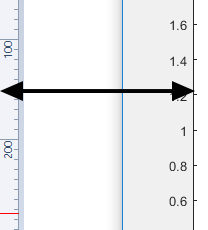
\includegraphics[scale=0.5]{fig1}
\par\end{centering}
\caption{Value of dist\_left.}
\end{figure}


\subsubsection{dist\_lower}
\begin{itemize}
\item Type: double.
\item Description: distance between the lower border of the drawing area
and the lower border of the screen.
\end{itemize}

\subsubsection{dist\_right}
\begin{itemize}
\item Type: double.
\item Description: distance between the right border of the drawing area
and the right border of the screen.
\end{itemize}

\subsubsection{dist\_upper}
\begin{itemize}
\item Type: double.
\item Description: distance between the upper border of the drawing area
and the upper border of the screen.
\end{itemize}

\subsection{Other outputs}

\subsection{Throwable custom exceptions}

\subsubsection{caller:DELETED\_FIGURE\_ERROR}
\begin{itemize}
\item Cause: an \texttt{InvalidHandle} exception has been thrown.
\item Error string: \texttt{The figure (drawing area) must not be closed
manually before the end of the running process.}
\end{itemize}

\subsection{Where it is used}
\begin{enumerate}
\item In online mode, at the first loop it is used by \texttt{start\_simulation}
before the simulation begins (the output values are used in the Simulink
model).\medskip{}
\medskip{}
\medskip{}
\medskip{}
\medskip{}
\end{enumerate}

\section{exit\_with\_error}

\subsection{Definition}

\texttt{function exit\_with\_error(id, errstr)}

\subsection{Brief description}

Closes all open resources, clears persistent variables in other internal
functions, opens a message box pointing the error out and throws an
exception in function of the parameters.

\subsection{Input parameters}

\subsubsection{id}
\begin{itemize}
\item Type: string.
\item Description: considering \texttt{caller:str2} as the exception-to-be-thrown's
identifier, this is \texttt{str2}.
\end{itemize}

\subsubsection{errstr}
\begin{itemize}
\item Type: string.
\item Description: the exception-to-be-thrown's error string.
\end{itemize}

\subsection{Output parameters}

\subsection{Other outputs}

\subsubsection{Message box}

An error message box is opened in the user's screen. The title has
the form \texttt{caller:id}; the message box text is \texttt{errstr}.

\subsection{Throwable custom exception}

\subsubsection{caller:id}
\begin{itemize}
\item Cause: call to \texttt{exit\_with\_error}.
\item Error string: \texttt{errstr.}
\end{itemize}

\subsection{Where it is used}

Every procedure that needs to exit after an error uses this function.\medskip{}
\medskip{}
\medskip{}
\medskip{}
\medskip{}


\section{get\_signals}

\subsection{Definition}

\texttt{function {[}xstar, xstardot, q1\_initial, q2\_initial{]} =
get\_signals(h\_step, tmin, tmax, xs, ys, l1, l2, sw)}

\subsection{Brief description}

Converts \texttt{xs} and \texttt{ys}, signals in a row vector format,
into a \texttt{{[}time; xs'; ys'{]}} format, where \texttt{time} is
the time column vector. Also returns the derivatives of \texttt{xs}
and \texttt{ys} in the same format and the initial angles needed for
the signal.

\subsection{Inputs description}

\subsubsection{h\_step}
\begin{itemize}
\item Type: double (positive).
\item Description: sampling step of \texttt{xs} and \texttt{ys}.
\end{itemize}

\subsubsection{tmin}
\begin{itemize}
\item Type: double.
\item Description: starting time of \texttt{xs} and \texttt{ys}.
\end{itemize}

\subsubsection{tmax}
\begin{itemize}
\item Type: double (greather than \texttt{tmin}).
\item Description: final time of \texttt{xs} and \texttt{ys}.
\end{itemize}

\subsubsection{xs}
\begin{itemize}
\item Type: row vector of doubles of size equal to that of \texttt{ys}.
\item Description: x component of the reference signal.
\end{itemize}

\subsubsection{ys}
\begin{itemize}
\item Type: row vector of doubles of size equal to that of \texttt{xs}.
\item Description: y component of the reference signal.
\end{itemize}

\subsubsection{l1}
\begin{itemize}
\item Type: double (positive).
\item Description: length of link 1 of the robot.
\end{itemize}

\subsubsection{l2}
\begin{itemize}
\item Type: double (positive).
\item Description: length of link 2 of the robot.
\end{itemize}

\subsubsection{sw}
\begin{itemize}
\item Type: integer (can be -1, 1 or 2).
\item Description: simulation switching parameter.
\end{itemize}

\subsection{Output parameters}

\subsubsection{xstar}
\begin{itemize}
\item Type: matrix of doubles.
\item Description: \texttt{{[}t xs' ys'{]}} where \texttt{t=(tmin:h:tmax)}'.
\end{itemize}

\subsubsection{xstardot}
\begin{itemize}
\item Type: matrix of doubles.
\item Description: \texttt{{[}t xsd' ysd'{]}} where \texttt{t=(tmin:h:tmax)}',
and \texttt{{[}xsd ysd{]}} is the numerical derivative of \texttt{{[}xs
ys{]}}, computed with Euler's method.
\end{itemize}

\subsubsection{q1\_initial}
\begin{itemize}
\item Type: double
\item Desctiption: initial value of q1 for the reference signal.
\end{itemize}

\subsubsection{q2\_initial}
\begin{itemize}
\item Type: double
\item Desctiption: initial value of q2 for the reference signal.
\end{itemize}

\subsection{Other outputs}

\subsection{Throwable custom exceptions}

\subsubsection{caller:INVALID\_INPUT\_SIZE\_ERROR}
\begin{itemize}
\item Cause: parameter sizes are not compatible.
\item Error string: \texttt{At least one component of the given reference
signal has invalid dimension. Each component must be a row vector
with floor((tmax-tmin)/h)+1 columns.}
\end{itemize}

\subsection{Where it is used}

In \texttt{prepare\_offline\_given} (to convert the user input into
the correct format) and in \texttt{prepare\_offline\_manual} (to convert
the \texttt{drawfreehand} output into the correct format).

\subsection{Notes}
\begin{itemize}
\item When executing the instruction \texttt{b=diff(a)}, where \texttt{a}
is an array of size \texttt{n}, \texttt{b} turns out to have \texttt{n
- 1} elements. This is because the \texttt{i}-th element of \texttt{b}
is computed as \texttt{b(i) = a(i+1)-a(i)}, and there is no \texttt{n
+ 1}-th element to use. Because of this, the last element of \texttt{xsd}
and \texttt{ysd} is computed separately: if the reference signal has
more than one sample, we use a backwards formula, \texttt{b(n) = a(n)-a(n-1)};
otherwise, the signal was a constant anyway, so we set the last (and
only) element to 0.
\end{itemize}
\medskip{}
\medskip{}
\medskip{}
\medskip{}
\medskip{}


\section{get\_simulation\_results}

\subsection{Definition}

\texttt{function {[}sim\_time, q1out, q2out, xout, yout, deltax, deltay{]}
= get\_simulation\_results(sw, q1q2, outs)}

\subsection{Brief description}

Takes the simulation results in the original Simulink format and converts
them into a column vector format.

\subsection{Input parameters}

\subsubsection{sw}
\begin{itemize}
\item Type: integer (can be -1, 1 or 2).
\item Description: simulation switching parameter.
\end{itemize}

\subsubsection{q1q2}
\begin{itemize}
\item Type: Simulink signal structure with two signals.
\item Description: robot generalized coordinates during the simulation.
\end{itemize}

\subsubsection{outs}
\begin{itemize}
\item Type: Simulink signal structure with six signals.
\item Description: components of actuator position, components of $\mathbf{\boldsymbol{\delta}x}$,
simulation variable \texttt{starting\_time}, and real time of the
simulation.
\end{itemize}

\subsection{Output parameters}

The output are those of \texttt{start\_simulation} (see I.2.4).

\subsection{Other outputs}

\subsection{Throwable exceptions}

\subsection{Where it is used}

In \texttt{start\_simulation}, after the end of each simulation.

\subsection{Notes}
\begin{itemize}
\item Call \texttt{sim\_time\_arr} the array of simulation times. In \texttt{OFFLINE}
modes, the values of the signals during the whole simulation run have
to be returned. On the other hand, in \texttt{ONLINE} mode, the results
that are to be considered are those after the initial conditions have
been reached; in this case, therefore, the only values that will be
returned are those with index $\ge$ \texttt{first\_time\_index},
where \texttt{first\_time\_index} is such that \texttt{sim\_time\_arr(first\_time\_index)}
is equal to the instant where the initial conditions are reached.
\end{itemize}
\medskip{}
\medskip{}
\medskip{}
\medskip{}
\medskip{}


\section{open\_figure}

\subsection{Definition}

\texttt{function f = open\_figure(sw, l1, l2)}

\subsection{Brief description}

Closes all open figures, opens and returns a new figure after applying
some customization for the simulation (see below).

\subsection{Input parameters}

\subsubsection{sw}
\begin{itemize}
\item Type: integer (can be -1, 1 or 2).
\item Description: simulation switching parameter.
\end{itemize}

\subsubsection{l1}
\begin{itemize}
\item Type: double (positive).
\item Description: length of link 1 of the robot.
\end{itemize}

\subsubsection{l2}
\begin{itemize}
\item Type: double (positive).
\item Description: length of link 2 of the robot.
\end{itemize}

\subsection{Output parameters}

\subsubsection{f}
\begin{itemize}
\item Type: figure handle.
\item Description: handles a figure with axis limits \texttt{{[}-(l1+l2),
l1+l2{]}} in both coordinates, maximized dimension, square shape if
not in online mode, \texttt{hold on} active, grid, pixel as axes units.
Furthermore, two (one if \texttt{l1 = l2}) circles are drawn in black,
respectively with radius \texttt{l1 + l2} and \texttt{abs(l1 - l2)}.
\end{itemize}

\subsection{Other outputs}

\subsubsection{f}

\texttt{f} is opened as well as returned.

\subsection{Throwable exceptions}

\subsection{Where it is used}
\begin{enumerate}
\item In \texttt{start\_simulation}, \texttt{prepare\_offline\_given}, \texttt{prepare\_offline\_manual},
it is called in order to open the simulation figure for the first
time.
\item In \texttt{plot\_robot\_position} and \texttt{start\_simulation},
it is called if it turns out the figure has been closed during simulation,
and must be re-opened.\medskip{}
\medskip{}
\medskip{}
\medskip{}
\medskip{}
\end{enumerate}

\section{plot\_mode\_str2int}

\subsection{Definition}

\texttt{function plot\_mode = plot\_mode\_str2int(plot\_mode)}

\subsection{Brief description}

Converts a valid plot mode string into an integer value.

\subsection{Input parameters}

\subsubsection{plot\_mode}
\begin{itemize}
\item Type: string (valid values: \texttt{NO\_PLOT}, \texttt{PLOT\_NO\_LINKS},
\texttt{PLOT\_WITH\_LINKS}).
\item Description: \texttt{NO\_PLOT} if no plot is desired during the simulation,
\texttt{PLOT\_NO\_LINKS} if only the plot of the robot position is
wanted, \texttt{PLOT\_WITH\_LINKS} if at each step the drawing of
the robot links are wanted.
\end{itemize}

\subsection{Output parameters}

\subsubsection{plot\_mode}
\begin{itemize}
\item Integer.
\item Description: 0 if input = \texttt{NO\_PLOT}, 1 if input = \texttt{PLOT\_NO\_LINKS},
2 if input = \texttt{PLOT\_WITH\_LINKS}.
\end{itemize}

\subsection{Other outputs}

\subsection{Throwable custom exceptions}

\subsubsection{caller:PLOT\_MODE\_ERROR}
\begin{itemize}
\item Cause: input has an invalid value.
\item Error string: \texttt{Given plot mode is not valid}.
\end{itemize}

\subsection{Where it is used}

At the beginning of \texttt{prepare\_simulation}.\medskip{}
\medskip{}
\medskip{}
\medskip{}
\medskip{}


\section{pos2angle}

\subsection{Definition}

\texttt{function {[}q1, q2{]} = pos2angle (x, y, l1, l2)}

\subsection{Brief description}

Given the actuator position and the length of the links, the corresponding
robot angles are returned.

\subsection{Input parameters}

\subsubsection{x}
\begin{itemize}
\item Type: double.
\item Desctiption: first component of actuator's position.
\end{itemize}

\subsubsection{y}
\begin{itemize}
\item Type: double.
\item Desctiption: second component of actuator's position.
\end{itemize}

\subsubsection{l1}
\begin{itemize}
\item Type: double (positive).
\item Desctiption: length of link 1 of the robot.
\end{itemize}

\subsubsection{l2}
\begin{itemize}
\item Type: double (positive).
\item Desctiption: length of link 2 of the robot.
\end{itemize}

\subsection{Output parameters}

\subsubsection{q1}
\begin{itemize}
\item Type: double.
\item Description: first generalized coordinate associated with \texttt{(x,
y}).
\end{itemize}

\subsubsection{q2}
\begin{itemize}
\item Type: double.
\item Description: second generalized coordinate associated with \texttt{(x,
y}).
\end{itemize}

\subsection{Other outputs}

\subsection{Throwable custom exceptions}

\subsection{Where it is used}

In \texttt{get\_signals} and \texttt{read\_cursor\_input}, in order
to compute the initial conditions for the Simulink model (if \texttt{x},
\texttt{y} are reachable).\medskip{}
\medskip{}
\medskip{}
\medskip{}
\medskip{}


\section{prepare\_offline\_given}

\subsection{Definition}

\texttt{function {[}n, q1\_initial, q2\_initial, xstar, xstardot,
sw{]}}

\texttt{= prepare\_offline\_given(l1, l2, h\_step, tmin, tmax, xs,
ys, plot\_mode)}

\subsection{Brief description}

In \texttt{OFFLINE\_GIVEN} mode, assigns 1 to n and \texttt{sw} and
computes the other output parameters through a call to \texttt{get\_signals}.
Afterwards, it opens a figure and plots the reference signal in red.

\subsection{Input, output parameters}

Input and output parameters are those of \texttt{prepare\_sim}, from
where this function is called in case the \texttt{OFFLINE\_GIVEN}
mode is requested.

\subsection{Other outputs}

\subsubsection{Figure}

A figure is opened through a call to \texttt{open\_figure}. The reference
signal is plotted on it in red, as an xy curve.

\subsection{Throwable custom exceptions}

\subsubsection{caller:ARG\_ERROR}
\begin{itemize}
\item Cause: \texttt{tmin > tmax}.
\item Error string: \texttt{tmin cannot be greater than tmax.}
\end{itemize}

\subsubsection{Other}

The exceptions throwable in \texttt{get\_signals} can be thrown.

\medskip{}
\medskip{}
\medskip{}
\medskip{}
\medskip{}


\section{prepare\_offline\_manual}

\subsection{Definition}

\texttt{function {[}n, q1\_initial, q2\_initial, tmin, tmax, xstar,
xstardot, sw{]}}

\texttt{= prepare\_offline\_manual(l1, l2)}

\subsection{Brief description}

In \texttt{OFFLINE\_MANUAL} mode, opens a figure and lets the user
draw an arbitrary number of continuous curves by using the \texttt{drawfreehand}
function. At the end of each drawing, a message asks the user if he/she
wants to draw another curve. The number of simulations and 1, respectively,
are assigned to \texttt{n} and \texttt{sw}.

\subsection{Input, output parameters}

Input and output parameters are those of \texttt{prepare\_sim}, from
where this function is called in case the \texttt{OFFLINE\_MANUAL}
mode is requested.

\subsection{Other outputs}

\subsubsection{Figure}

A figure is opened through call to \texttt{open\_figure} if \texttt{plot\_mode}
is positive.

\subsubsection{Message box}

At the end of each drawing, a message box asks the user if he/she
wants to draw another curve.

\subsection{Throwable custom exceptions}

\subsubsection{caller:DELETED\_FIGURE\_ERROR}
\begin{itemize}
\item Cause: a \texttt{MATLAB:class:InvalidHandle} exception is thrown by
the \texttt{drawfreehand} function as a result of closing the figure
during the drawing process.
\item Error string: \texttt{The figure (drawing area) must not be closed
manually before the end of the running process.}
\end{itemize}

\subsubsection{Others}

The exceptions throwable in \texttt{get\_signals} can be thrown.

\subsection{Notes}
\begin{itemize}
\item To obtain the curve drawn by the user, a call to \texttt{drawfreehand},
a MATLAB system function, is performed. Since this function returns
all the plotted points after the call has terminated, i.e. after the
plot is completed, it could not be used in the \texttt{ONLINE} mode,
where the drawn points are needed as soon as possible by the simulator.
However, it was decided to use it here, and not to use the custom
routine implemented for the \texttt{ONLINE} mode, as \texttt{drawfreehand}
is more precise and more performing.
\item If the figure is closed during the simulation, \texttt{drawfreehand}
returns a null object; therefore the process has to be stopped with
error (see 11.5.1).
\end{itemize}
\medskip{}
\medskip{}
\medskip{}
\medskip{}
\medskip{}


\part{Simulink model documentation}

After an introduction, each of the following sections is associated
to an area of the Simulink model.

\section{Introduction}

The model uses a set of variables; each one is associated to a GOTO
block. In particular, \texttt{l1}, \texttt{l2}, \texttt{sw}, \texttt{vmax},
\texttt{tmin}, \texttt{plot\_mode} are used in all modes with obvious
role.

The variable \texttt{starting\_time} is computed at every step in
the Achievement of initial position area, and holds value \texttt{tmin}
in \texttt{OFFLINE} modes; in \texttt{ONLINE} mode, it has value -1
before the initial conditions are reached, and their time of achievement
afterwards.

The variable \texttt{reset} is computed at every step in the Reference
signal acquisition area, and is always valued 0 in \texttt{OFFLINE}
modes. In \texttt{ONLINE} mode, it is valued 0 before the user has
started drawing, and 1 afterwards.

The variable \texttt{ended} is computed at every step in the Reference
signal acquisition area, and is valued 0 before the simulation has
ended, 1 afterwards. Since the non-abnormal end of the simulation
is issued as an input of 1 to the \texttt{STOP} block, this parameter
can be used by the other areas in the remaining execution of the last
step of simulation.

IMPORTANT: the Simulink model is run from the \texttt{start\_simulation}
function (through a call to the \texttt{sim} function), and the simulation
parameters, including the simulation step, are given as parameters
there. HOWEVER, don't put different settings in the Simulink configuration
parameters settings. For example, calling \texttt{sim} with a fixed
step parameter AND setting the solver to \texttt{auto} in the solver
configuration parameters settings will cause Simulink to set as actual
simulation step the GCD of the \texttt{sim} parameter and a Simulink-generated
step. This WILL cause confusion, so be careful.

\section{Initial assignments area}

\begin{figure}[h]
\begin{centering}
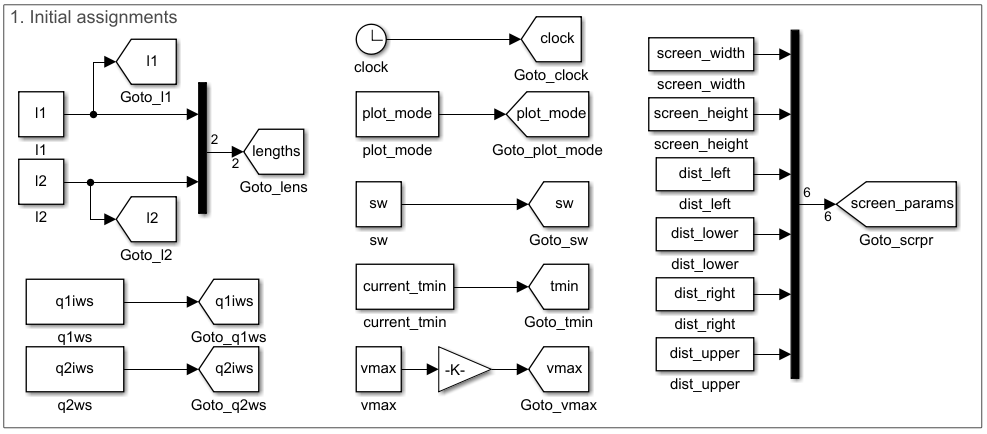
\includegraphics[scale=0.55]{simulink1assign}
\par\end{centering}
\caption{Initial assignments8 area.}
\end{figure}

In this area several parameters (\texttt{l1}, \texttt{l2}, \texttt{q1ws},
\texttt{q2ws}, \texttt{clock}, \texttt{plot\_mode}, \texttt{sw}, \texttt{current\_tmin},
\texttt{vmax} and all the screen parameters) from the workspace are
assigned to a \texttt{GOTO} block. This way, if one or moreof those
parameters get their name changed in a future development of the software,
the model has to be changed in one place only. Observe that \texttt{vmax}
is multiplied by a scaling gain, different from 1 only in modes 2
and 3.

\medskip{}
\medskip{}
\medskip{}
\medskip{}


\section{Reference signal acquisition area}

\begin{figure}[H]
\begin{centering}
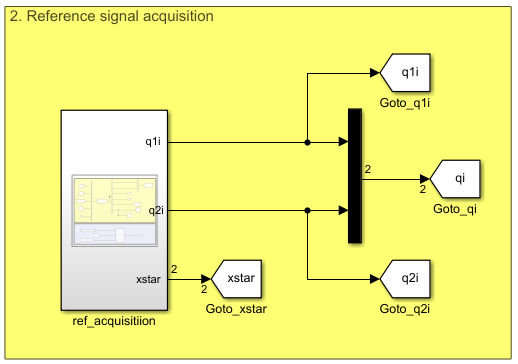
\includegraphics[scale=0.65]{simulink2refac}
\par\end{centering}
\caption{Reference signal acquisition.}
\end{figure}

The \texttt{ref\_acquisition }subsystem is composed of two areas:
the Online reference processing area and the Choice of Reference area.

\subsection{Online reference processing area}

\begin{figure}[H]
\begin{centering}
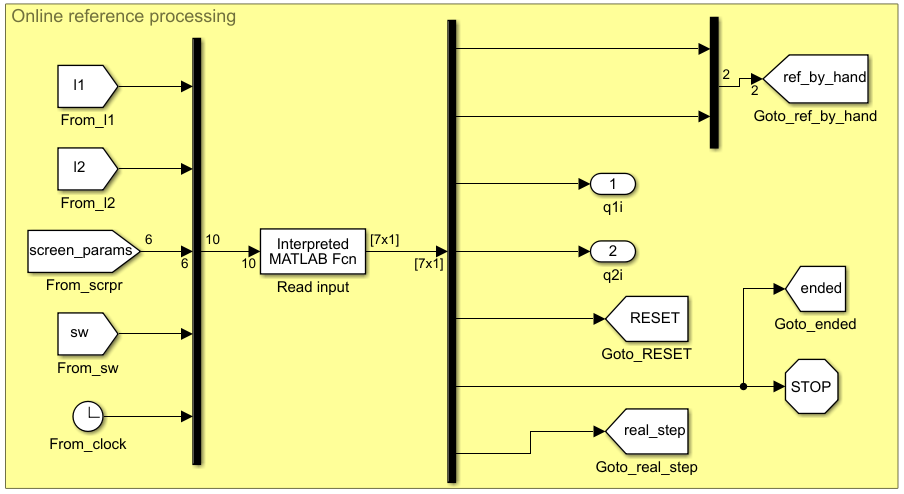
\includegraphics[scale=0.45]{simulink2refac_online}
\par\end{centering}
\caption{\texttt{ref\_acquisition} subsystem.}
\end{figure}

In \texttt{ONLINE} mode, this area reads and stores the cursor input
in the \texttt{GOTO} block \texttt{ref\_by\_hand}, as well as assigning
a few other variables (see 1.4.1.1).

\subsubsection{MATLAB interpreted function read\_cursor\_input}

\paragraph{Definition}

\noindent \texttt{function out = read\_cursor\_input (in)}.

\paragraph{Output parameters}

\noindent The output signal \texttt{out} is a column array of size
6. In \texttt{OFFLINE} modes, this function is not used, therefore
the outputs always have a value of 0. In \texttt{ONLINE} mode, its
elements are the following (listed from first to last):
\begin{itemize}
\item \texttt{xstar}, \texttt{ystar} = zero vector before the user starts
drawing; the two components of the reference signal, provided by the
user through the use of the cursor, afterwards.
\item \texttt{q1i}, \texttt{q2i} = respectively 0 and 4 (arbitrary values)
before the user starts drawing; the initial angles associated with
the reference signal drawn by the user after the user has started
drawing.
\item \texttt{RESET} = 0 before the user starts drawing, 1 afterwards. The
change of value of this variable happens the first time that the mouse
results clicked and the clicked point is inside the drawing area.
\item \texttt{ended} = 0 before the simulation has terminated, 1 afterwards.
The change of value of this variable happens if the mouse is not clicked
and \texttt{RESET} is equal to 1, i.e. the mouse has been released
by the user.
\end{itemize}

\paragraph{Other outputs}

\noindent After the user has started drawing, i.e. when \texttt{RESET
> 0}, the points provided by the user through the cursor are plotted
in red on the opened simulation figure.

\paragraph{Custom exceptions}

\noindent An exception of id \texttt{caller:FIRST\_POINT\_NOT\_REACHABLE\_ERROR}
and error string \texttt{First point of the reference signal is not
reachable.} can be thrown if the first point plotted by the user is
outside of the reachability space.

\paragraph{Note}

At implementation time, a convenient way to capture the position of
the cursor at each instant was seeked. Consider the command \texttt{get(gca,
'CurrentPoint');}; it returns the cursor's coordinates with respect
to the current axes, but only returns the last clicked or unclicked
point, ignoring the points over which the cursor hovered. Oddly enough,
the command \texttt{get(0, 'PointerLocation');} returns the points
with respect to the screen coordinates, but at all times, not only
when the user clicks or unclicks. The second instruction is therefore
used; however, the obtained point must be converted to the figure/axes
coordinates, and this is the reason for which the values computed
by \texttt{compute\_screen\_parameters} are provided as input to \texttt{read\_cursor\_input}.
The formulas to convert the points were obtained through a simple
transformation of coordinates.

For instance, consider the x coordinate. Define $L\coloneqq l_{1}+l_{2}$,
$d_{L}\coloneqq$ \texttt{dist\_left}, $d_{R}\coloneqq$ \texttt{dist\_right},
$w\coloneqq$\texttt{screen\_width}. To transform the value $x_{s}$
(relative to screen coordinates) to $x_{a}$ (relative to axes coordinates),
we need the straight line going through the points ($x_{s}=d_{L}$,
$x_{a}=-2L$) and ($x_{s}=w-d_{R}$, $x_{a}=2L$), that is, the straight
line satisfying the equations
\begin{center}
$-2L=m_{x}d_{L}+q_{x}$
\par\end{center}

\begin{center}
$2L=m_{x}(w-d_{R})+q_{x}$
\par\end{center}

Solving for $m_{x}$ and $q_{x}$ easily gives $m_{x}=\frac{4L}{w-d_{R}-d_{L}},q_{x}=-2L-\frac{4L}{w-d_{R}-d_{L}}d_{L}$,
which are the relationships used in the program (rearranged in order
to avoid multiple computations of $\frac{4L}{w-d_{R}-d_{L}}$). For
the y coordinate, an analogous procedure (or noticing the simmetry
of the problem) yields $m_{y}=\frac{4L}{h-d_{D}-d_{U}},q_{y}=-2L-\frac{4L}{h-d_{D}-d_{U}}d_{D}$,
where $h$ = \texttt{screen\_height}, $d_{D}$ = \texttt{dist\_lower},
$d_{U}$ = \texttt{dist\_upper}.

\subsection{Choice of reference area}

\begin{figure}[H]
\begin{centering}
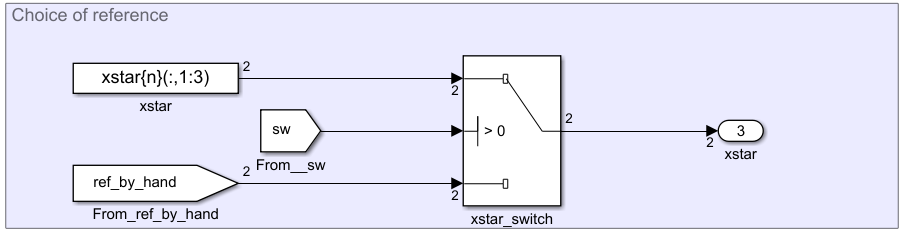
\includegraphics[scale=0.5]{simulink2refac_choice}
\par\end{centering}
\caption{Choice of reference area.}
\end{figure}

In \texttt{ONLINE} mode, this area assigns the \texttt{ref\_by\_hand
}signal (the cursor input) to \texttt{xstar}; in \texttt{OFFLINE}
modes, the \texttt{n}-th cell of \texttt{xstar} (workspace variable)
is assigned instead.

\medskip{}
\medskip{}
\medskip{}
\medskip{}
\medskip{}


\section{xstardot computation area}

\begin{figure}[H]
\begin{centering}
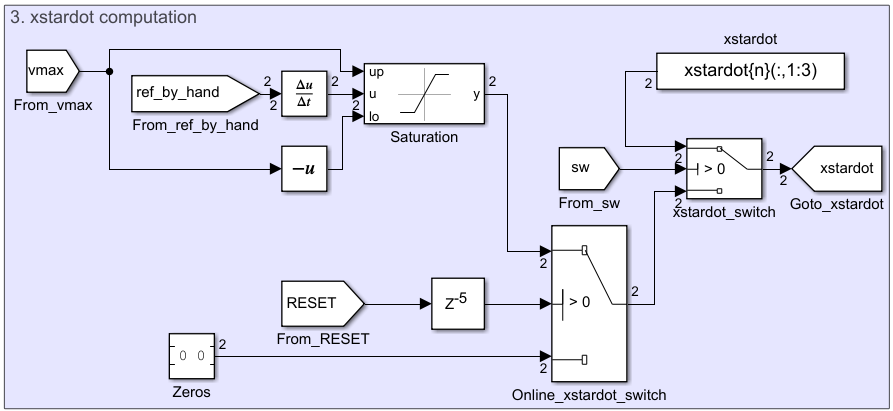
\includegraphics[scale=0.6]{simulink3xstardot}
\par\end{centering}
\caption{xstardot computation area.}
\end{figure}
This area selects the derivative of the reference. If \texttt{sw}
> 0, the n-th element of the workspace cell array \texttt{xstardot}
is trivially chosen. In the other case, it is more complicated.

For now, ignore the delay block. Before \texttt{RESET} is set to a
positive value, i.e. before the user has started drawing, a null derivative
is provided (any finite signal would do, as this part is going to
be ignored). Roughly after \texttt{RESET} changes sign, a saturated
version of the derivative of the hand(cursor)-drawn reference signal
is provided instead.

The saturation allows the simulation not to crash on the user when
the latter exceeds the maximum speed of the robot (however, the robot
will proceed at its maximum velocity, forcing the user to slow down).
Finally, the delay block is necessary because, when the user starts
drawing, a jump will happen, i.e. the derivative of the cursor-drawn
signal will be very high. We want the robot to start as still, so
we provide null derivative for a few more time steps.

\section{qdot computation area}

\begin{figure}[h]
\begin{centering}
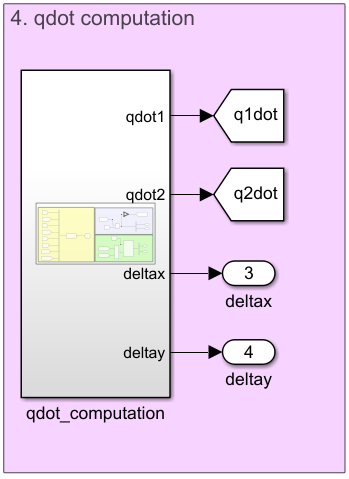
\includegraphics[scale=0.5]{simulink4qdot}
\par\end{centering}
\caption{qdot computation area.}
\end{figure}

The \texttt{qdot\_computation} subsystem faithfully implements the
robot control logic seen in the introduction. Internally, it has three
areas: the Inversion of J area, the K$\times$Deltax computation area
and the Final computation area.

\begin{figure}[h]
\begin{centering}
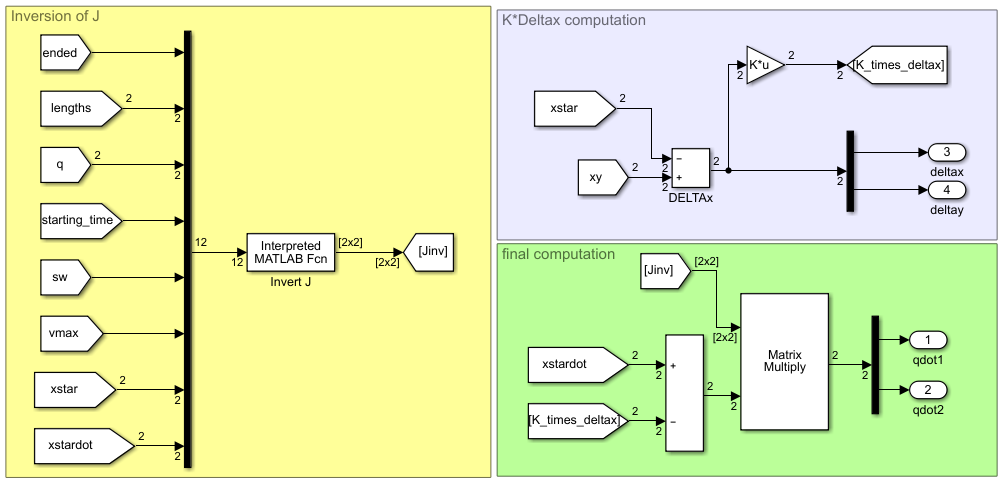
\includegraphics[scale=0.45]{simulink4qdot_sub}
\par\end{centering}
\caption{qdot\_computation subsystem}
\end{figure}

As said, the calculations are those explained in the introduction.

\subsubsection{Interpreted MATLAB function invert\_J}

If inputs \texttt{xstar}, \texttt{ystar}, \texttt{xstardot} and \texttt{ystardot}
specify a valid signal (that is, not exceeding maximum speed \texttt{vmax}
and being reachable), the output is the inverse of the Jacobian of
the system. Otherwise, an exception is thrown; it can be of two types:
\begin{enumerate}
\item id = \texttt{caller:MAX\_SPEED\_EXCEEDED\_ERROR}, error text = \texttt{Maximum
speed exceeded.}
\item id = \texttt{caller:POINT\_NOT\_REACHABLE\_ERROR}, error text = \texttt{Point
is not reachable.}
\end{enumerate}

\section{Arm area}

\begin{figure}[h]
\begin{centering}
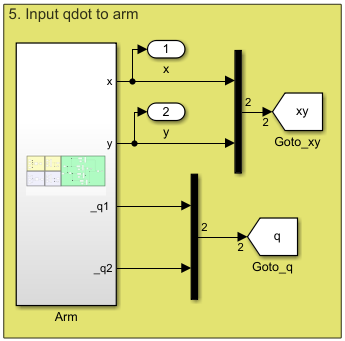
\includegraphics[scale=0.6]{simulink5arm}
\par\end{centering}
\caption{Arm area.}
\end{figure}

The Arm subsystem uses \texttt{qdot}, computed in the qdot computation
area, to calculate the actuator's position (multiplexed into \texttt{xy})
and the associated angles (multiplexed into \texttt{q}).

\subsection{Arm subsystem}

\begin{figure}[H]
\begin{centering}
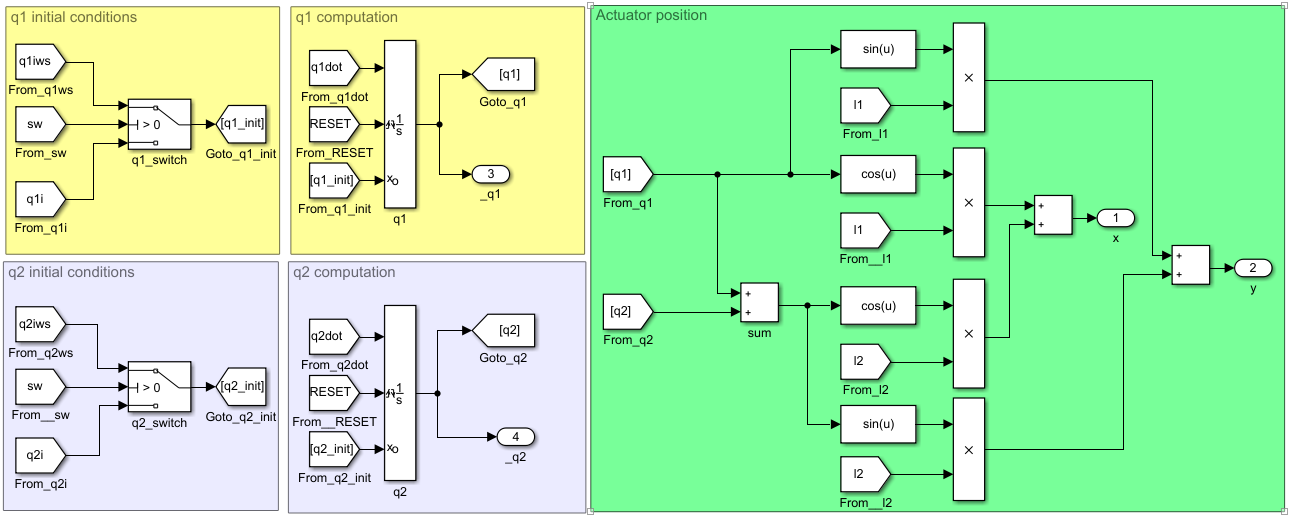
\includegraphics[scale=0.5]{simulink5armarm}
\par\end{centering}
\caption{Arm subsystem.}
\end{figure}


\subsubsection{Initial conditions areas}

The two leftmost areas select the correct initial angles. If \texttt{sw}
> 0, i.e. the simulation is in an \texttt{OFFLINE} mode, the signals
\texttt{q1i} and \texttt{q2i}, computed during the simulation in the
Reference signal acquisition area, are chosen. Otherwise, the signals
\texttt{q1iws} and \texttt{q2iws}, computed before the simulation
in the workspace, are chosen.

\subsubsection{Angles computation}

The remaining areas perform the integration of the derivatives of
\texttt{q1} and \texttt{q2}, in order to obtain \texttt{q1} and \texttt{q2},
which are then returned as third and fourth outputs.

The integrators reset to the initial condition signals \texttt{q1\_init}
and \texttt{q2\_init} when the signal \texttt{RESET} changes sign;
in the \texttt{OFFLINE} modes this never happens, while in the \texttt{ONLINE}
mode this happens after the user has started drawing, and \texttt{q1\_init},
\texttt{q2\_init} have been assigned to the needed initial angles
by the \texttt{read\_user\_input} function (see 17.1).

\subsubsection{Actuator position area}

This area outputs the components of the actuator's position, \texttt{x}
and \texttt{y}, after being computed from the angles \texttt{q1} and
\texttt{q2} according to the relationships
\begin{center}
$x=l_{1}\mathrm{cos}q_{1}+l_{2}\mathrm{cos}(q_{1}+q_{2})$
\par\end{center}

\begin{center}
$y=l_{1}\mathrm{sin}q_{1}+l_{2}\mathrm{sin}(q_{1}+q_{2})$
\par\end{center}

\medskip{}
\medskip{}
\medskip{}
\medskip{}
\medskip{}


\section{Time handling area}

\begin{figure}[h]
\begin{centering}
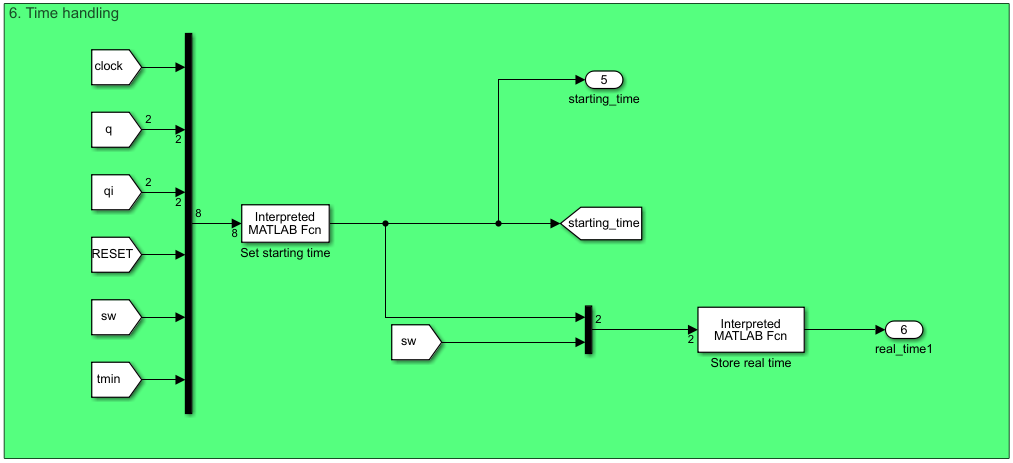
\includegraphics[scale=0.55]{simulink6time_handling}
\par\end{centering}
\caption{Achievement of initial position area.}
\end{figure}


\subsection{MATLAB interpreted function set\_starting\_time}

\subsubsection{Definition}

\texttt{function starting\_time = set\_starting\_time(in)}

\subsubsection{Output parameters}
\begin{enumerate}
\item \texttt{starting\_time} = \texttt{tmin} in \texttt{OFFLINE} modes.
In \texttt{ONLINE} mode, \texttt{starting\_time} = -1 if the initial
condition have yet to be reached; otherwise, \texttt{starting\_time}
= the instant in which they have been reached. In \texttt{ONLINE}
mode, the value of \texttt{starting\_time} is used in the other parts
of the model to determine if the initial condition have been reached.
\end{enumerate}

\subsubsection{Other outputs}

\subsubsection{Throwable custom exceptions}

\subsection{Interpreted MATLAB function store\_real\_time}

\subsubsection{Definition}

\texttt{function t = store\_real\_time (in)}

\subsubsection{Output parameters}
\begin{enumerate}
\item \texttt{t} = 0 in mode 1 (this output is not significant). In mode
2, \texttt{t = toc}. In mode 3, \texttt{t = toc} if \texttt{tic} has
been called (i.e. \texttt{starting\_time} $\ge$ 0, see 14.1), otherwise
\texttt{t =} 0.
\end{enumerate}

\subsubsection{Other outputs}

\subsubsection{Throwable custom exceptions}

\subsubsection{Notes}
\begin{itemize}
\item In the \texttt{OFFLINE} modes, \texttt{set\_starting\_times} runs
\texttt{tic} at the first simulation step, so \texttt{store\_toc}
(which executes after \texttt{set\_starting\_times} as it needs its
output as input) can execute the \texttt{toc} command always. In \texttt{ONLINE}
mode, \texttt{tic} is only run by \texttt{set\_starting\_times} at
the step where initial conditions have been reached, so \texttt{toc}
can't be executed until then, and 0 will be returned instead.
\end{itemize}
\medskip{}
\medskip{}
\medskip{}
\medskip{}
\medskip{}


\section{Plot area}
\begin{center}
\begin{figure}[H]
\begin{centering}
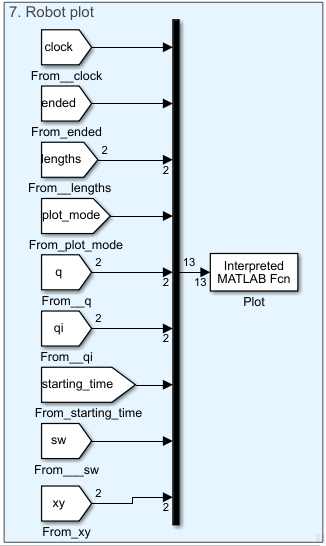
\includegraphics[scale=0.5]{simulink7plot}
\par\end{centering}
\caption{Plot area.}
\end{figure}
\par\end{center}

\subsection{MATLAB interpreted function plot\_robot\_position}

\subsubsection{Definition}

\texttt{function plot\_robot\_position(in)}

\subsubsection{Output parameters}

\subsubsection{Other outputs}
\begin{itemize}
\item If \texttt{plot\_mode = 1} (and, in \texttt{ONLINE} mode, if \texttt{starting\_time}
$\ge$ 0), the function plots, in blue, a straight line that goes
from the previous position of the actuator to the current one, if
the two positions are different; it draws a point if they are equal,
and at the first step (when a ``previous position'' doesn't exist).
\item If \texttt{plot\_mode = 2} (and, in \texttt{ONLINE} mode, if \texttt{starting\_time}
$\ge$ 0), the function plots, at every step, two lines in the position
of the robot's links, in blue. It also deletes the links drawn at
the previous step, if any.
\item Otherwise, it does nothing.
\item If the figure is closed by the user while the simulation is running
and \texttt{plot\_mode} is not 0, the function re-opens the figure
and issues a warning, with message \texttt{It is recommended not to
close the figure during the simulation.}
\end{itemize}

\subsubsection{Throwable custom exceptions}

\subsubsection{Notes}

\paragraph{Note 1}

This function, when plotting is enabled, is the bottleneck of the
whole simulator, and dominates the execution time. For example, with
$t_{min}=0$, $t_{max}=6$ s, $h_{step}=0.001$, $\mathbf{x}^{*}(t)=(0.7\mathrm{cos}(10t),0.7\mathrm{sin}(10t)+0.01)$,
$v_{max}=100$, $l_{1}=1$, $l_{2}=0.8$, the simulation takes:
\begin{itemize}
\item 10.931683 seconds with \texttt{plot\_mode = PLOT\_WITH\_LINKS}.
\item 10.247887 seconds with \texttt{plot\_mode = PLOT\_NO\_LINKS}.
\item 1.670445 seconds with \texttt{plot\_mode = NO\_PLOT}.
\end{itemize}
Although qualitatively, these results show the fact that the plotting
heavily affects the running time. To avoid even more overhead, in
the case of \texttt{plot\_mode = PLOT\_WITH\_LINKS} the two links
are plotted through a single instruction.

\paragraph{Note 2}

This function uses a local persistent variable, \texttt{plotted},
to store the latest element plotted in the figure in \texttt{PLOT\_WITH\_LINKS}
plot mode. At each call, if the variable is not empty, i.e. after
the first links configuration is plotted, the command \texttt{delete(plotted)}
is issued, in order to erase the previous links configuration plot.

In \texttt{start\_simulation}, after each simulation, the functions
that use persistent variables are cleared (i.e. their persistent variables
are reset to empty values), except for this one. This is because,
after the end of a simulation, if there is a next one plotted will
contain the latest links configuration of the previous simulation,
and will be automatically erased.

Note that the command \texttt{clear plot\_robot\_position} must be
issued before \texttt{start\_simulation} returns (and, in case of
error exit, in \texttt{exit\_with\_error}, too).\medskip{}
\medskip{}
\medskip{}
\medskip{}
\medskip{}


\part{Examples of use}

\section{Example 1}

\noindent \texttt{tmin=-0.1; tmax=1; h\_step=0.001; t=tmin:h\_step:tmax;}

\noindent \texttt{sim\_struct = prepare\_simulation('OFFLINE\_GIVEN',
'PLOT\_NO\_LINKS', 1, 1, 0.8, h\_step, tmin, tmax, 0.6{*}cos(t), 0.6{*}sin(t));}

Output:

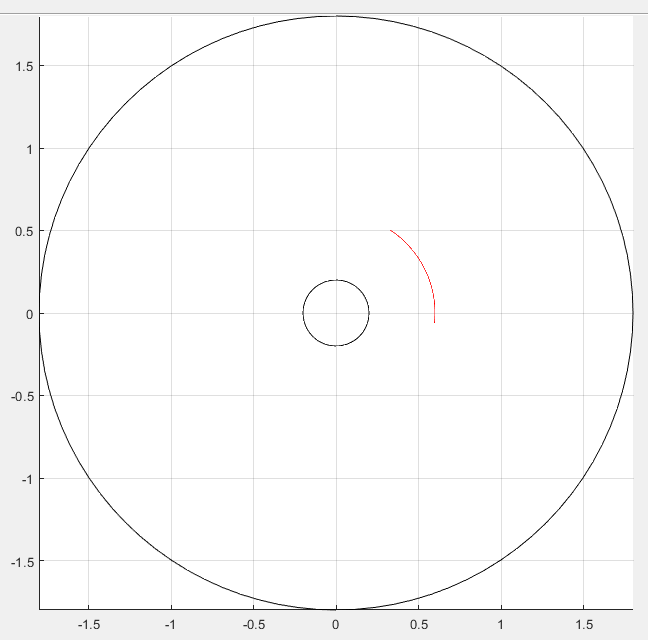
\includegraphics[scale=0.5]{run1fig1}
\noindent \begin{flushleft}
\texttt{{[}t, q1, q2, x, y, deltax, deltay{]} = start\_simulation(sim\_struct);}
\par\end{flushleft}

Output:

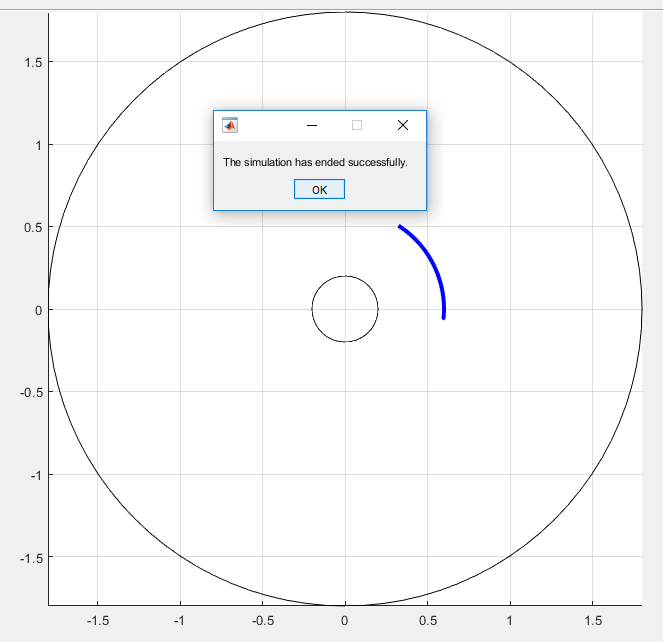
\includegraphics[scale=0.5]{run1fig2}

\noindent \texttt{figure(2); plot(x\{1\}, y\{1\});}

Output:

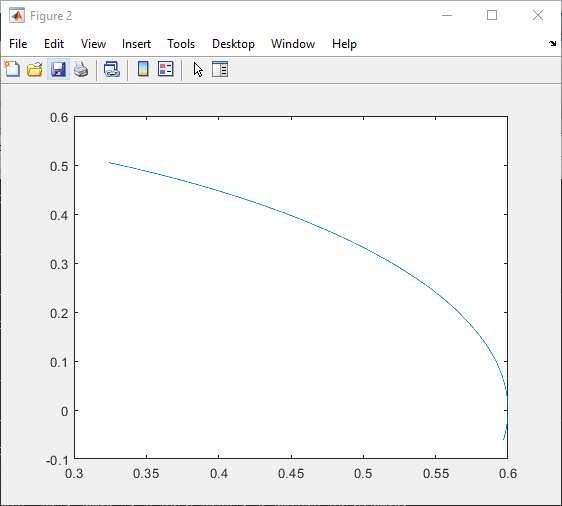
\includegraphics[scale=0.7]{run1fig3}

\section{Example 2}

\noindent \texttt{sim\_struct = prepare\_simulation('OFFLINE\_MANUAL',
'PLOT\_WITH\_LINKS', 1, 1, 0.8, 0.001);}

Output:

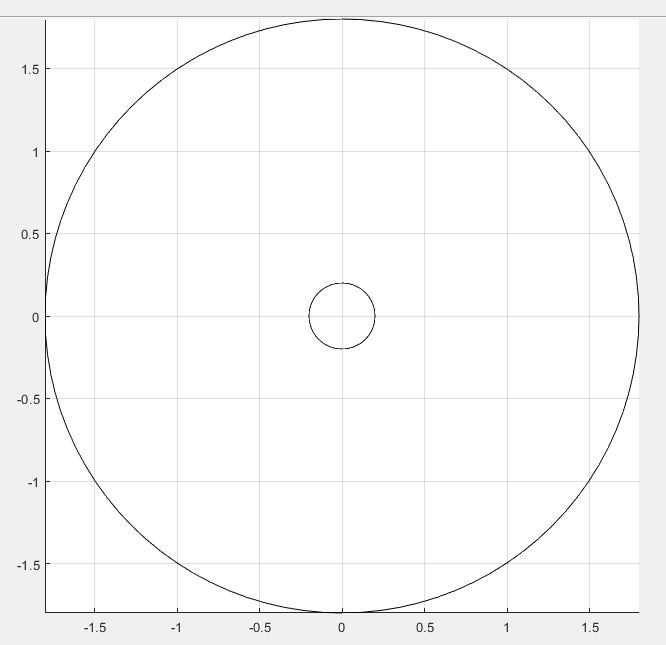
\includegraphics[scale=0.5]{run2fig1}

After drawing one signals:

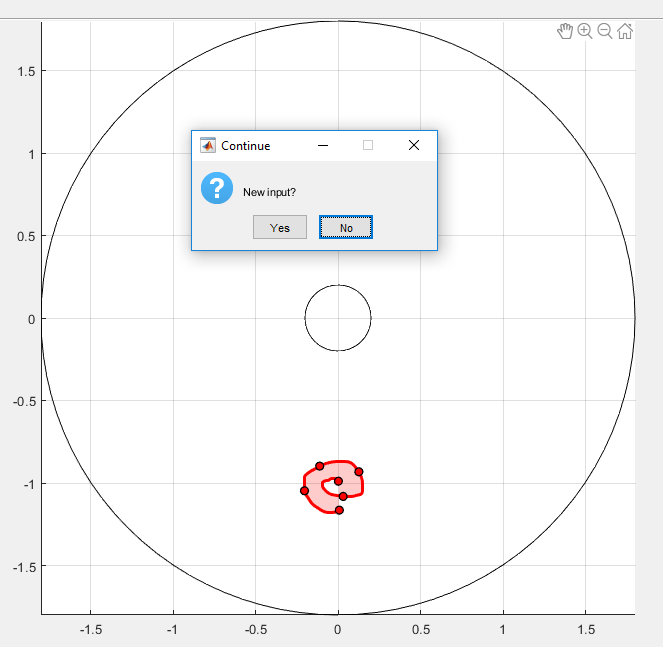
\includegraphics[scale=0.5]{run2fig2}

After choosing ``Yes'', drawing another signal and choosing ``No'':

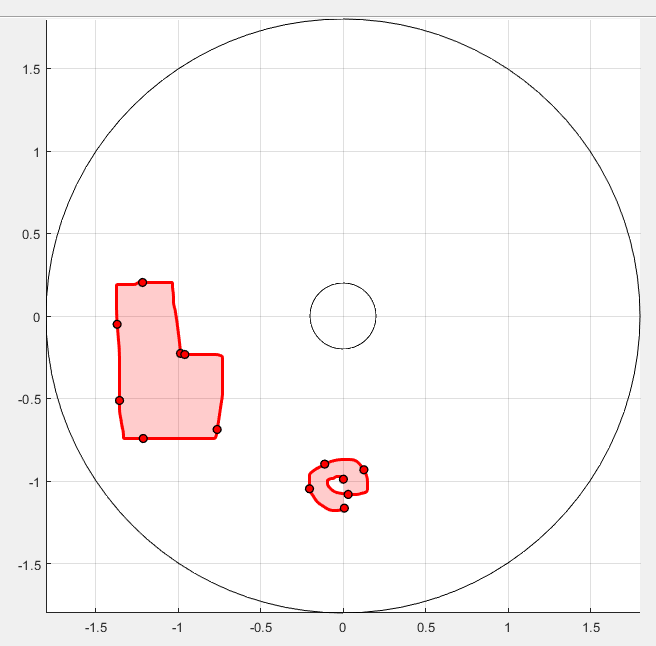
\includegraphics[scale=0.5]{run2fig3}
\noindent \begin{flushleft}
\texttt{{[}t, q1, q2, x, y, deltax, deltay{]} = start\_simulation(sim\_struct);}
\par\end{flushleft}

While plotting:

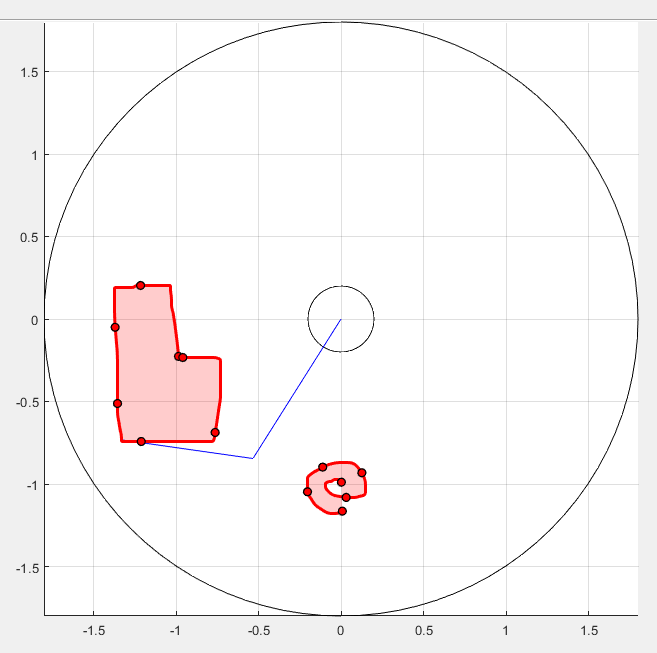
\includegraphics[scale=0.59]{run2fig4}

\noindent \texttt{figure(2); hold on; grid on; axis({[}-2 2 -2 2{]});
plot(x\{1\}, y\{1\}, x\{2\}, y\{2\});}

Output:

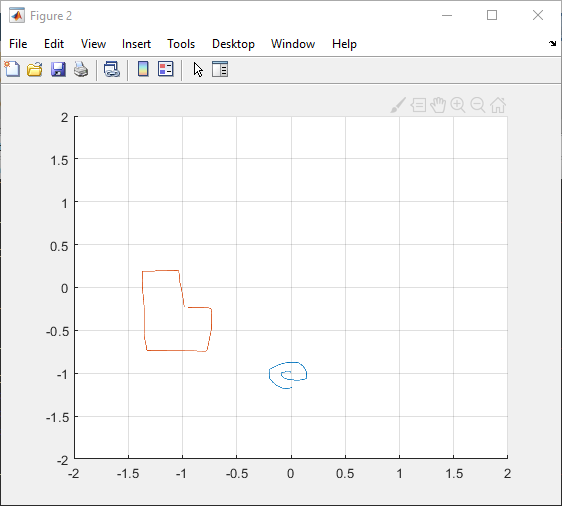
\includegraphics[scale=0.7]{run2fig5}

\section{Example 3}

\texttt{sim\_struct = prepare\_simulation('ONLINE', 'PLOT\_NO\_ARM',
1, 1, 0.8, 0.00001);}

\noindent \texttt{{[}t, q1, q2, x, y, deltax, deltay{]} = start\_simulation(sim\_struct);}

Output after plotting some curves:

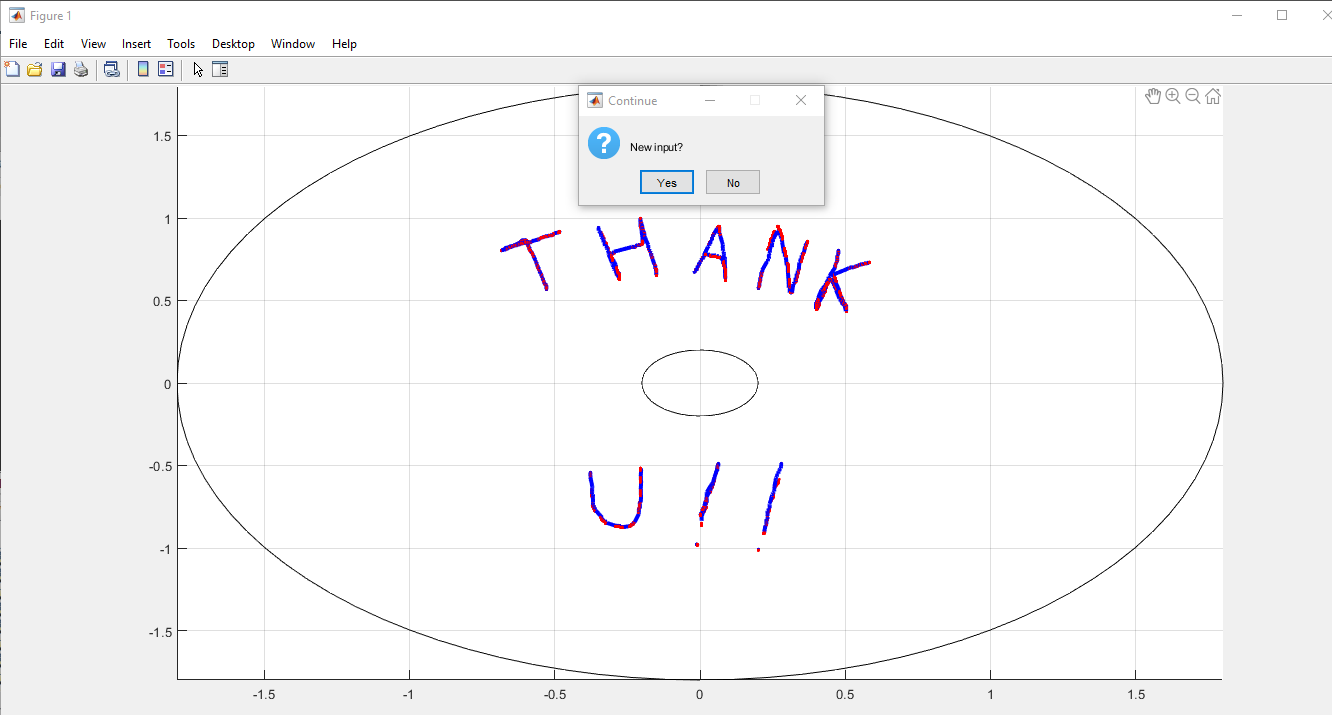
\includegraphics[scale=0.5]{run3fig1}

\noindent \texttt{figure(2); hold on; for ii = 1 : max(size(x)) plot(x\{ii\},
y\{ii\},'.-'); end}

Output:

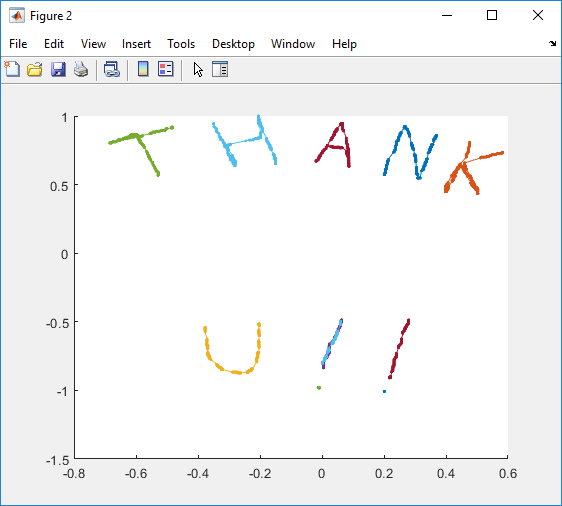
\includegraphics[scale=0.7]{run3fig2}
\end{document}
